\chapter{工具trait}\label{ch13}

\emph{Science is nothing else than the search to discover unity in the wild variety of nature—or, more exactly, in the variety of our experience. Poetry, painting, the arts are the same search, in Coleridge’s phrase, for unity in variety.}

\begin{flushright}
    ——Jacob Bronowski
\end{flushright}

这一章将介绍Rust中的“工具” trait,它们是标准库中能够显著影响到编写Rust代码的方式的trait,因此你需要熟悉它们才能写出惯用的代码并设计出你的用户会觉得是“Rustic”的crate接口。它们可以分为三大类:

\codeentry{语言扩展trait}
\hangparagraph{正如我们上一章介绍的运算符重载trait可以让你对自己的类型使用Rust的表达式运算符,还有几个其他的标准库trait充当Rust的扩展,让你可以把自己的类型更紧密地集成到语言中。这一类包括\texttt{Drop}、\texttt{Deref}和\texttt{DerefMut},以及转换用的trait \texttt{From}和\texttt{Into}。我们将在本章介绍所有这些trait。}

\codeentry{标记trait}
\hangparagraph{有几个trait通常用于约束泛型类型变量来表达一些特殊的约束。这一类包括\texttt{Sized}和\texttt{Copy}。}

\codeentry{公开的词汇表trait}
\hangparagraph{这些trait并没有神秘的编译器集成,你可以在自己的代码中定义等价的trait。但它们服务于为常见问题制定常规解决方案的重要目标。这些trait在crate和模块之间的公共接口中特别有价值:通过减少不必要的变化,它们让接口更容易理解,它们还增加了不同crate的特性可以简单地集成在一起的可能性,并且无需样板或自定义的粘合代码。这一类包括\texttt{Default}、引用借用trait \texttt{AsRef}、\texttt{AsMut}、\texttt{Borrow}、\texttt{BorrowMut},可能失败的转换 trait\texttt{TryFrom}和\texttt{TryInto},以及\texttt{ToOwned} trait,它是\texttt{Clone}的泛化。}

\hyperref[t13-1]{表13-1}是对它们的总结。

\begin{table}[htbp]
    \centering
    \caption{工具trait汇总}
    \label{t13-1}
    \begin{tabular}{p{0.2\textwidth}p{0.9\textwidth}}
        \hline
        \textbf{trait}  & \textbf{说明} \\
        \hline

        \nameref{drop}  & 析构器。当一个值被drop时Rust会自动运行的清理代码。    \\
        \rowcolor{tablecolor}
        \nameref{sized} & 标记trait,标记一个类型有一个编译期已知的固定大小,与动态大小的类型(例如切片)相反。 \\
        \nameref{clone} & 支持克隆的类型。  \\
        \rowcolor{tablecolor}
        \nameref{Copy}  & 标记trait,标记一个类型可以通过按位拷贝包含值的内存来克隆新值。   \\
        \nameref{deref} & 为智能指针类型准备的trait。   \\
        \rowcolor{tablecolor}
        \nameref{default}   & 有一个有意义的“默认值”的类型。    \\
        \nameref{asref} & 用于从一个类型的值借用另一个类型的引用的转换trait。   \\
        \rowcolor{tablecolor}
        \nameref{borrow}& 转换trait,类似于\texttt{Asref/AsMut},但额外保证一致的哈希性、顺序性和相等性。   \\
        \nameref{from}  & 用于将一个类型的值转换为另一个类型的值的转换trait。   \\
        \rowcolor{tablecolor}
        \nameref{tryfrom}   & 用于将一个类型的值转换为另一个类型的值的转换trait,用于可能失败的转换。   \\
        \nameref{toowned}   & 将一个引用转换为一个有所有权的值的转换trait。 \\
    \end{tabular}
\end{table}

还有一些其它重要的标准库trait。我们将在\hyperref[ch15]{第15章}中介绍\texttt{Iterator}和\texttt{IntoIterator}。用于计算哈希值的\texttt{Hash} trait,将在\hyperref[ch16]{第16章}中介绍。还有一对标记线程安全类型的trait,\texttt{Send}和\texttt{Sync},将在\hyperref[ch19]{第19章}中介绍。

\section{\texttt{Drop}}\label{drop}

当一个值的所有者消失时,我们说Rust \emph{drop}了这个值。drop一个值意味着释放这个值拥有的所有其他值、堆上的存储空间和系统资源。drop会在各种情况下发生:当变量离开作用域时、处于表达式语句的末尾时、截断vector时从尾部移除元素时,等等。

在大多数情况下,Rust自动为你处理drop过程。例如,假设你定义了下面的类型:
\begin{minted}{Rust}
    struct Appellation {
        name: String,
        nicknames: Vec<String>
    }
\end{minted}

一个\texttt{Appellation}拥有为字符串内容和vector的元素缓冲区分配的堆上的空间。当一个\texttt{Appellation}被drop时,Rust会清理所有这些内容,你不需要编写任何代码。然而,如果你想的话,你可以通过实现\texttt{std::ops::Drop} trait来自定义Rust如何drop你的类型的值:
\begin{minted}{Rust}
    trait Drop {
        fn drop(&mut self);
    }
\end{minted}

\texttt{Drop}的实现类似于C++中的析构函数,或者其它语言中的终结函数。当一个值被drop时,如果它实现了\texttt{std::ops::Drop},Rust会在清理它的字段或元素之前先调用它的\texttt{drop}方法。这种\texttt{drop}的隐式调用是唯一一种调用这个方法的方式,如果你尝试显式地调用这个方法,Rust会标记为错误。

因为Rust会在drop一个值的字段或方法之前先用这个值调用\texttt{Drop::drop},所以这个方法接收到的值总是保持完全初始化的状态。我们的\texttt{Appellation}类型的一个\texttt{Drop}的实现可以充分利用它的字段:
\begin{minted}{Rust}
    impl Drop for Appellation {
        fn drop(&mut self) {
            print!("Dropping {}", self.name);
            if !self.nicknames.is_empty() {
                print!(" (AKA {})", self.nicknames.join(", "));
            }
            println!("");
        }
    }
\end{minted}

有了这个实现,我们可以写出下列代码:
\begin{minted}{Rust}
    {
        let mut a = Appellation {
            name: "Zeus".to_string(),
            nicknames: vec!["cloud collector".to_string(),
                            "king of the gods".to_string()]
        };

        println!("before assignment");
        a = Appellation { name: "Hera".to_string(), nicknames: vec![] };
        println!("at end of block");
    }
\end{minted}

当我们把第二个\texttt{Appellation}赋给\texttt{a}的时候,第一个值会被drop,当我们离开\texttt{a}的作用域时,第二个值也会被drop。这段代码会打印出如下内容:
\begin{minted}{text}
    before assignment
    Dropping Zeus (AKA cloud collector, king of the gods)
    at end of block
    Dropping Hera
\end{minted}

因为我们的\texttt{Appellation}的\texttt{std::ops::Drop}实现只打印了一条消息,那么它的内存到底是怎么被精确地清理掉的?\texttt{Vec}类型也实现了\texttt{Drop},drop它的每个元素,然后释放在堆上分配的缓冲区。一个\texttt{String}在内部使用\texttt{Vec<u8>}来保存文本,因此\texttt{String}自身没有实现\texttt{Drop},它让它的\texttt{Vec}来清理字符。同样的规则也适用于\texttt{Appellation}值:当一个值被drop时,它的\texttt{Vec}的\texttt{Drop}实现负责清理每一个字符串的内容,并最终释放存储元素的缓冲区。保存\texttt{Appellation}值的内存本身也有一个拥有者,可能是一个局部变量或者一些数据结构,它们负责释放它。

如果一个变量的值被移动走,导致当它离开作用域时是未初始化的状态,那么Rust会避免drop这个变量:它里面没有值可以drop。即使按照控制流一个变量的值可能被移动走、也可能没有的情况下,这个原则也会生效。Rust会使用一个不可见的标记来追踪变量的状态,它指示变量的值是否需要被drop:
\begin{minted}{Rust}
    let p;
    {
        let q = Appellation { name: "Cardamine hirsuta".to_string(),
                              nicknames: vec!["shotweed".to_string(),
                                              "bittercress".to_string()] };
        if complicated_condition() {
            p = q;
        }
    }
    println!("Sproing! What was that?");
\end{minted}

根据\texttt{complicated\_condition}返回\texttt{true}还是\texttt{false},\texttt{p}或者\texttt{q}最后将会拥有这个\texttt{Appellation},另一个变为未初始化。这个值最终落在哪个变量里决定了它会在\texttt{println!}之前还是之后被drop。因为\texttt{q}在\texttt{println!}之前离开作用域,而\texttt{p}在之后。尽管一个值可能会被移来移去,但Rust只会drop它一次。

你通常不需要实现\texttt{std::ops::Drop},除非你想定义一个拥有一些Rust不知道的资源的类型。例如,在Unix系统上,Rust的标准库内部使用下面的类型来表示一个操作系统文件描述符:
\begin{minted}{Rust}
    struct FileDesc {
        fd: c_int,
    }
\end{minted}

\texttt{FileDesc}的\texttt{fd}字段就是当程序使用完它之后应该被关闭的文件描述符的序号。\texttt{c\_int}是\texttt{i32}的一个别名。标准库中按照如下方式为\texttt{FileDesc}实现了\texttt{Drop}:
\begin{minted}{Rust}
    impl Drop for FileDesc {
        fn drop(&mut self) {
            let _ = unsafe { libc::close(self.fd) };
        }
    }
\end{minted}

这里,\texttt{libc::close}是C库中的\texttt{close}函数的Rust名称。Rust代码只能在\texttt{unsafe}块中调用C函数,因此这里标准库使用了\texttt{unsafe}块。

如果一个类型实现了\texttt{Drop},它就不能再实现\texttt{Copy}。如果一个类型是\texttt{Copy}的,那意味着按位复制就可以创建一个新的独立拷贝。但通常在同样的数据上调用同一个\texttt{drop}方法不止一次是一个错误。

标注prelude中包含了一个drop值的函数\texttt{drop},但它的定义一点也不神奇:
\begin{minted}{Rust}
    fn drop<T>(_x: T) { }
\end{minted}

换句话说,它以值接收参数,从调用者那里获取所有权——然后什么也不做。当\texttt{\_x}离开作用域时Rust会drop它的值,正如它对其他任何变量做的一样。

\section{\texttt{Sized}}\label{sized}

\emph{固定大小的类型(sized type)}是指那些所有实例值都占用相同大小的内存空间的类型。Rust中几乎所有的类型都是固定大小的:每一个\texttt{u64}都是8字节,每一个\texttt{(f32, f32, f32)}类型的值都占12个字节。即使枚举也是固定大小的:不管它当前实际的variant是哪一个,一个枚举总是占用能存下最大的variant的空间。即使\texttt{Vec<T>}拥有一个大小可变的堆上缓冲区,\texttt{Vec}值本身的大小就是一个缓冲区的指针,加上容量,加上长度。因此\texttt{Vec<T>}是一个固定大小的类型。

所有的固定大小的类型都实现了\texttt{std::marker::Sized} trait,它没有任何方法或关联类型。Rust为所有适合的类型自动实现它,你不能自己实现它。\texttt{Sized}唯一的用途是作为类型参数的约束:一个类似\texttt{T: Sized}的约束要求\texttt{T}是一个大小在编译期已知的类型。这种类型的trait被称为\emph{标记trait(marker trait)},因为Rust语言本身使用它们来标记有特定特点的类型。

然而,Rust还有少量\emph{大小不固定的类型(unsized type)},它们的值的大小并不相同。例如,字符串切片类型\texttt{str}(注意,没有\&)就是大小不固定的。字符串\texttt{"diminutive"}和\texttt{"big"}分别是占用了10个和3个字节的\texttt{str}切片的引用。如\hyperref[f13-1]{图13-1}所示。数组切片类型例如\texttt{[T]}(再次注意,这里也没有\&)也是大小不固定的:一个共享引用例如\texttt{\&[u8]}可以指向一个任意大小的\texttt{[u8]}切片。因为\texttt{str}和\texttt{[T]}类型表示不同大小的值的集合,因此它们是大小不固定的类型。

\begin{figure}[htbp]
    \centering
    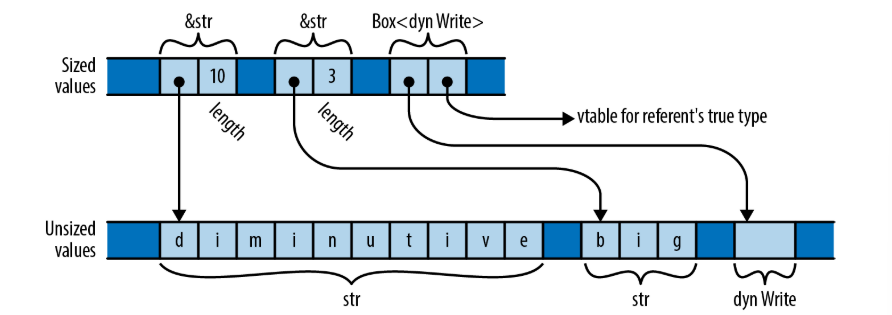
\includegraphics[width=0.8\textwidth]{../img/f13-1.png}
    \caption{指向大小不固定的值的引用}
    \label{f13-1}
\end{figure}

Rust中另一种常见的大小不固定类型是\texttt{dyn}类型,它是trait对象引用的目标。正如我们在“\nameref{traitobject}”中解释的一样,一个trait对象是一个指向实现了给定trait的值的指针。例如,类型\texttt{\&dyn std::io::Write}和\texttt{Box<dyn std::io::Write>}是指向实现了\texttt{Write} trait的值的指针。被引用的目标可能是一个文件或者网络套接字,或者是实现了\texttt{Write}的自定义类型。因为实现了\texttt{Write}的类型的集合是开放的,所以\texttt{dyn Write}也是大小不固定的类型:它的值可能有任意的大小。

Rust不能在变量中存储大小不固定的值或者将它们传递为参数。你只能通过指针例如\texttt{\&str}或\texttt{Box<dyn Write>}来处理它们,指针本身是固定大小的。正如\hyperref[f13-1]{表13-1}所示,一个指向大小不固定的值的指针总是一个\emph{胖指针(fat pointer)},占用两个字节:一个指向切片的指针加上切片的长度、一个trait对象加上一个指向方法实现的vtable的指针。

trait对象和切片的指针是对称的。在这两种情况下,都缺乏相应的类型信息:你不能在不知道\texttt{[u8]}长度的情况下索引它,也不能在不知道被指向的值的具体\texttt{Write}实现的情况下调用\texttt{Box<dyn Write>}的方法。在这两种情况下,胖指针填充了类型缺失的信息,加上了一个长度或者vtable的指针。被省略的静态信息被替换为了动态信息。

因为大小不固定的类型限制太多,所以大多数泛型类型参数都被限制为\texttt{Sized}类型。事实上,它几乎总是必须的,因此在Rust中它是默认的:如果你写\texttt{struct S<T> \{ ... \}},Rust认为你的意思是\texttt{struct S<T: Sized> \{ ... \}}。如果你不让\texttt{T}有这个约束,你必须显式写出来,即\texttt{struct S<T: ?Sized> \{ ... \}}。\texttt{?Sized}语法专门用于这种场景,含义是”不需要是\texttt{Sized}“。例如,如果你写了\texttt{struct S<T: ?Sized> \{ b: Box<T> \}},那么Rust将允许你写\texttt{S<Str>}和\texttt{S<dyn Write>},这时\texttt{b}将是一个胖指针;而\texttt{S<i32>}和\texttt{S<String>}中,\texttt{b}是一个普通指针。

抛开它们的限制不谈,大小不固定的类型让Rust的类型系统工作得更加顺畅。如果阅读标准库的文档,你偶尔会看到类型参数中的\texttt{?Sized}约束,这几乎总是意味着给定的类型只能被指向,同时允许相关的代码既能处理普通类型、又能处理切片和trait对象。当一个类型参数有\texttt{?Sized}约束时,人们通常会说它是\emph{可能大小不固定(questionably sized)}:它可能是\texttt{Sized},也可能不是。

除了切片和trait对象之外,还有另一种大小不固定的类型。一个结构体的最后一个字段(也只有最后一个字段)可能是大小不固定的,那么这个结构体本身也是大小不固定的。例如,\texttt{Rc<T>}引用计数指针内部被实现为私有类型\texttt{RcBox<T>}的指针,它存储了\texttt{T}和引用计数。这里有一个\texttt{RcBox}的简化版的定义:
\begin{minted}{Rust}
    struct RcBox<T: ?Sized> {
        ref_count: usize,
        value: T,
    }
\end{minted}

\texttt{value}字段就是\texttt{Rc<T>}引用的\texttt{T}值,\texttt{Rc<T>}解引用之后就是一个这个字段的指针。\texttt{ref\_count}字段保存引用计数。

真正的\texttt{RcBox}是标准库的实现细节,不能用于公开使用。但假设我们在处理一个上面的定义。你可以将\texttt{RcBox}和固定大小的类型一起使用,例如\texttt{RcBox<String>},结果将是一个固定大小的结构体类型。或者你可以将它和大小不固定的类型一起使用,例如\texttt{RcBox<dyn std::fmt::Display>}(其中\texttt{Display}表示可以被\texttt{println!}以及类似的宏格式化的类型),\texttt{RcBox<dyn Display>}是一个大小不固定的结构体类型。

你不能直接创建一个\texttt{RcBox<dyn Display>}值。你必须先创建一个普通的、固定大小的\texttt{RcBox},它的\texttt{value}字段的类型需要实现\texttt{Display},例如\texttt{RcBox<String>}。然后Rust允许你把一个它的引用\texttt{\&RcBox<String>}转换为胖指针引用\texttt{\&RcBox<dyn Display>}:
\begin{minted}{Rust}
    let boxed_lunch: RcBox<String> = RcBox {
        ref_count: 1,
        value: "lunch".to_string()
    };

    use std::fmt::Display;
    let boxed_displayable: &RcBox<dyn Display> = &boxed_lunch;
\end{minted}

当向函数传递参数时会隐式发生这个转换,因此你可以向接受\texttt{\&RcBox<dyn Display>}参数的函数传递一个\texttt{\&RcBox<String>}:
\begin{minted}{Rust}
    fn display(boxed: &RcBox<dyn Display>) {
        println!("For your enjoyment: {}", &boxed.value);
    }

    display(&boxed_lunch);
\end{minted}

这将会产生下列输出:
\begin{minted}{text}
    For your enjoyment: lunch
\end{minted}

\section{\texttt{Clone}}\label{clone}

\texttt{std::clone::Clone} trait用于那些可以拷贝自身的类型。\texttt{Clone}的定义如下:
\begin{minted}{Rust}
    trait Clone: Sized {
        fn clone(&self) -> Self;
        fn clone_from(&mut self, source: &Self) {
            *self = source.clone()
        }
    }
\end{minted}

\texttt{clone}方法应该构建一个\texttt{self}的独立拷贝并返回它。因为这个方法的返回类型是\texttt{Self},并且函数不能返回大小不固定的值,因此\texttt{Clone} trait扩展了\texttt{Sized} trait:它会约束实现的\texttt{Self}类型是\texttt{Sized}。

拷贝一个值通常意味着拷贝它拥有的所有内容,因此\texttt{clone}可能在时间和内存上的开销都比较大。例如,克隆一个\texttt{Vec<String>}不止要拷贝vector,还要拷贝它的每一个\texttt{String}元素。这就是为什么Rust不会自动拷贝值,而是要求你显式地调用方法来拷贝。引用计数指针例如\texttt{Rc<T>}和\texttt{Arc<T>}是例外:拷贝它们只会简单地递增引用计数并返回给你一个新的指针。

\texttt{clone\_from}方法将\texttt{self}修改为\texttt{source}的拷贝。\texttt{clone\_from}的默认实现简单地拷贝\texttt{source},然后将它移动进\texttt{*self}。这总是能正确工作,当对于某些类型,还有更快的方法达成相同的效果。例如,假设\texttt{s}和\texttt{t}都是\texttt{String}。语句\texttt{s = t.clone();}必须先克隆\texttt{t},drop掉\texttt{s}的旧值,然后将克隆的值移动进\texttt{s},因此这里面有一次堆分配和堆释放。但如果\texttt{s}原本的堆缓冲区有足够的容量存下\texttt{t}的内容,那么没有必要进行释放和分配操作:可以简单地将\texttt{t}的文本拷贝进\texttt{s}的缓冲区,然后调整它的长度。在泛型代码中,你应该使用\texttt{clone\_from},这样可以充分利用优化过的实现的优势。

如果你的类型的\texttt{Clone}实现只是简单地调用每一个字段或者元素的\texttt{clone}方法,然后利用这些克隆的值构造一个新的值,那么\texttt{clone\_from}的默认定义就已经够了,Rust将会为你实现它:只要在类型的定义上方加上\texttt{\#[derive(Clone)]}。

标准库中几乎所有应该能拷贝的类型都实现了\texttt{Clone}。基本类型例如\texttt{bool}和\texttt{i32}实现了。容器类型例如\texttt{String, Vec<T>, HashMap}也实现了。一些不应该能拷贝的类型例如\texttt{std::sync::Mutex}没有实现\texttt{Clone}。一些类型例如\texttt{std::fs::File}可以拷贝,但如果操作系统没有足够的资源那么拷贝可能会失败,这些类型也没有实现\texttt{Clone},因为\texttt{clone}不允许失败。作为替代,\texttt{std::fs::File}提供了一个\texttt{try\_clone}方法,它返回一个\texttt{std::io::Result<File>}来报告失败。

\section{\texttt{Copy}}\label{Copy}

在\hyperref[ch04]{第4章}中,我们解释过,对于大多数类型,赋值操作会移动它的值,而不是拷贝它们。移动值让我们可以更容易地追踪它们拥有的资源。但在“\nameref{copy}”中,我们指出了例外情况:不持有任何资源的简单类型可以是\texttt{Copy}类型,这种类型的赋值操作会拷贝源值,而不是移动值并把源值设为未初始化。

那个时候,我们并没有确切地说明\texttt{Copy}到底是什么,但现在我们可以告诉你:如果一个类型实现了\texttt{std::marker::Copy}标记trait,那么它就是\texttt{Copy}的,\texttt{Copy}的定义如下:
\begin{minted}{Rust}
    trait Copy: Clone { }
\end{minted}

很容易就可以为你自己的类型实现它:
\begin{minted}{Rust}
    impl Copy for MyType { }
\end{minted}

但因为\texttt{Copy}是一个有特殊含义的标记trait,所以Rust只允许可以通过逐字节的浅拷贝来拷贝自身的类型实现\texttt{Copy}。如果一个类型拥有任何其他资源,例如堆缓冲区或者操作系统句柄,那么它将不能实现\texttt{Copy}。

任何实现了\texttt{Drop} trait的类型不能实现\texttt{Copy}。Rust假定如果一个类型需要特殊的清理代码,那么它肯定也需要特殊的拷贝代码,所以不能是\texttt{Copy}。

和\texttt{Clone}一样,你可以使用\texttt{\#[derive(Copy)]}来让Rsut为你实现\texttt{Copy}。你通常能一次性看到它们两个,即\texttt{\#[derive(Copy, Clone)]}。

在将类型变为\texttt{Copy}之前请仔细思考。尽管这样做会让类型更容易使用,但却对类型本身的实现添加了很大的限制。而且隐式的拷贝可能会有很大的开销。我们已经在“\nameref{copy}”中详细解释了这些因素。

\section{\texttt{Deref}与\texttt{DerefMut}}\label{deref}

\section{\texttt{Default}}\label{default}

\section{\texttt{AsRef}与\texttt{AsMut}}\label{asref}

\section{\texttt{Borrow}与\texttt{BorrowMut}}\label{borrow}

\section{\texttt{From}与\texttt{Into}}\label{from}

\section{\texttt{TryFrom}与\texttt{TryInto}}\label{tryfrom}

\section{\texttt{ToOwned}}\label{toowned}
